\documentclass[11pt,a4paper]{article}

\usepackage[utf8]{inputenc} 
\usepackage[T1]{fontenc} 
\usepackage{lmodern}
\usepackage[margin=2cm]{geometry}
\usepackage[german]{babel}
\usepackage{amsmath} 
\usepackage{graphicx} 
\usepackage{booktabs}
\usepackage{hyperref}
\hypersetup{
    colorlinks,
    citecolor=red,
    filecolor=black,
    linkcolor=black!20!blue!90!,
    urlcolor=black} 
\usepackage{nicefrac}
\usepackage[table]{xcolor}
\usepackage{tocloft}
\usepackage[section]{placeins}

\setlength{\parindent}{0pt}
\setlength{\parskip}{1ex plus 0.5ex minus 0.5ex}

\definecolor{incolor}{rgb}{0.0, 0.0, 0.5}

\hbadness=99999

\newcommand{\refpy}[1]{Siehe Anhang: \textit{Rechnungen in Python} (\texttt{{\color{incolor}In [{\color{incolor}#1}]}})}
\newcommand\dif{\mathop{}\!\mathrm{d}}
\newcommand{\halftime}[4]{\begin{figure}[h]
\begin{minipage}{.#1\textwidth}#3\end{minipage}\begin{minipage}{.#2\textwidth}
\centering
#4\end{minipage}
\end{figure}}
\renewcommand{\vec}{\boldsymbol}

\begin{document}


{
\centering 
\large 
Physiklabor für Anf\"anger*innen \\
Ferienpraktikum im Sommersemester 2018 \\[4mm]
\textbf{\LARGE 
Versuch 75: Lichtmikroskop
} \\[3mm]
(durchgef\"uhrt am 01.10.2018 bei Daniel Bartel) \\
Gruppe 14: Andréz Gockel, Patrick M\"unnich\\
\today \\[10mm]
}

\vspace{50pt}
\tableofcontents
\vspace{22pt}

\pagebreak

\section{Ziel des Versuchs}

\begin{enumerate}
\item Aufbau des Köhlerschen Beleuchtungsstrahlengangs
\item Aufbau des Objektivs, Messung des Abbildungsma\ss stabs am Zwischenbild
\item Separater Aufbau des Okulars, Messung der Okularvergr\"o\ss rung
\item Kombination zum Mikroskopstrahlengang, Messung der Gesamtvergr\"o\ss erung 
\item \textbf{bonus} Begrenzung des Aufl\"osungsverm\"ogens durch einen Spalt im Strahlengang 
\item \textbf{bonus} Beobachtung von Linsenfehlern, Vergleich mit kommerziellen Mikroskopen
\end{enumerate}


\section{Physikalische Zusammenh"ange}

Die wahrgenommene Gr"o\ss e eines Gegenstands h"angt von der Gr"o\ss e des Bilds $B$ und der Bildweite $b$ ab:
\begin{equation}
\epsilon_0=\arctan\left(\frac{B}{b}\right)\label{eq:1}
\end{equation}
Wird ein Objekt durch eine Lupe betrachtet, so h"angt die Vergr"o\ss erung des Gegenstands $G$ von dem Abstand $f$ dessen zur Lupe und der als 250\,mm definierten Bezugssehweite ab:
\begin{equation}
V_{Lupe}\approx\frac{\tan\epsilon}{\tan\epsilon_0}=\frac{\nicefrac{G}{f}}{\nicefrac{G}{s_0}}=\frac{s_0}{f}\label{eq:3}
\end{equation}
Das ganze wird komplizierter, wenn wie statt einer Lupe ein Lichtmikroskop verwenden. Wir gehen von einem aus zwei Sammellinsen bestehendes Mikroskop aus. Das hei\ss t, dass zuerst durch ein Objektiv ein vergr"o\ss erndes Zwischenbild erzeugt wird und dann durch ein Okular das Resultat angeschaut wird. Das Zwischenbild hat die Gr"o\ss e $B$ und wird mit dem Abbildungsma\ss stab
\begin{equation}
\beta=\frac{B}{G}=\frac{b}{g}\label{eq:4}
\end{equation}
erzeugt. Im Okular wird dies unter dem Sehwinkel $\epsilon\approx\tan\left(\frac{B}{f_{Ok}}\right)$ betrachtet. Unsere Gesamtvergr"o\ss erung sieht dann folgenderma\ss en aus:
\begin{equation}
V_M=\frac{\epsilon}{\epsilon_0}=\frac{\nicefrac{B}{f_2}}{\nicefrac{G}{s_0}}=\frac{b}{g}\frac{s_0}{f_2}=\beta_{Obj}V_{Ok}\label{eq:5}
\end{equation}

Wichtig ist auch zu verstehen, dass es immer eine Aufl"osebegrenzung gibt, d.h. man kann nicht unendlich klein sehen. Um dies zu berechnen, f"uhren wir erstmal die numerische Apertur NA ein. Dieser Wert h"angt sowohl von de halben "Offnungswinkel des Objektivs $\alpha$ als auch von der Brechzahl der Immersionsfl"ussigkeit $n$ ab:
\begin{equation}
\mathrm{NA}=n\sin\alpha\label{eq:7}
\end{equation}
Ohne Immersionsfl"ussigkeit ist immer NA$<1$, mit einer ist NA$\geq1.4$.
Um daraus unser Abbe-Kriterium f"ur den kleinsten noch aufl"osbaren Abstand zu finden rechnen wir dann
\begin{equation}
\delta=\frac{1.22\lambda}{2\mathrm{NA}}=\frac{1.22\lambda}{2n\sin\alpha}\label{eq:8}
\end{equation}

\section{Aufbau}

Für diesen Versuch wird eine optische Bank mit austauschbaren und verschiebbaren optischen Komponenten verwendet. Es stehen sämtliche Komponente zur verfügung:
\begin{itemize}
	\item LED Leuchte
	\item 4 Linsen
	\begin{itemize}
		\item Kollektorlinse ($f_1$ = 40\,mm)
		\item Kondensorlinse ($f_2$ = 40\,mm)
		\item Objektiv ($f_3$ = 40\,mm)
		\item Okular ($f_4$ = 80\,mm)
	\end{itemize}
	\item 2 Blenden
	\begin{itemize}
		\item Leuchtfeldblende
		\item Aperaturblende
	\end{itemize}
	\item 2 Objekte
	\begin{itemize}
	\item Dia mit einem Gitter
	\item Dia mit einer Mikrometerskala
	\end{itemize}
	\item 2 Bildschirme
	\begin{itemize}
	\item Eine weiße Mattscheibe mit aufgedruckter Mikrometerskala auf einer Seite
	\item Eine semi-transparente Mattscheibe  
	\end{itemize}
	\item Verstellbarere Spalt
	\item Strahlteiler
	\item Beleuchteter Referenzmaßstab
\end{itemize}
Zusätzlich werden ein Massband, und ein Geodreieck für die Messungen verwendet. 

Das Objektiv ist in diesem Versuch mit einem flachen Stab mit der Bildschirmhalterung verbunden, sodass dieser abstand immer gleich ist (wie bei einem kommerziellen Mikroskop). Die Lichtquelle ist am linken Ende der Bank fixiert und der beleuchtete Referenzmaßstab an dem rechten Ende. Zu begin wird das Objektiv mit dem weißen Schirm in der Halterung so verschoben, dass die Lichtquelle gut auf dem Schirm abgebildet wird. 

Für den letzten Teil steht steht auch ein kommerzielles Mikroskop mit diversen Preperaten zur verfügung.


\begin{figure}
\centering
{\fbox{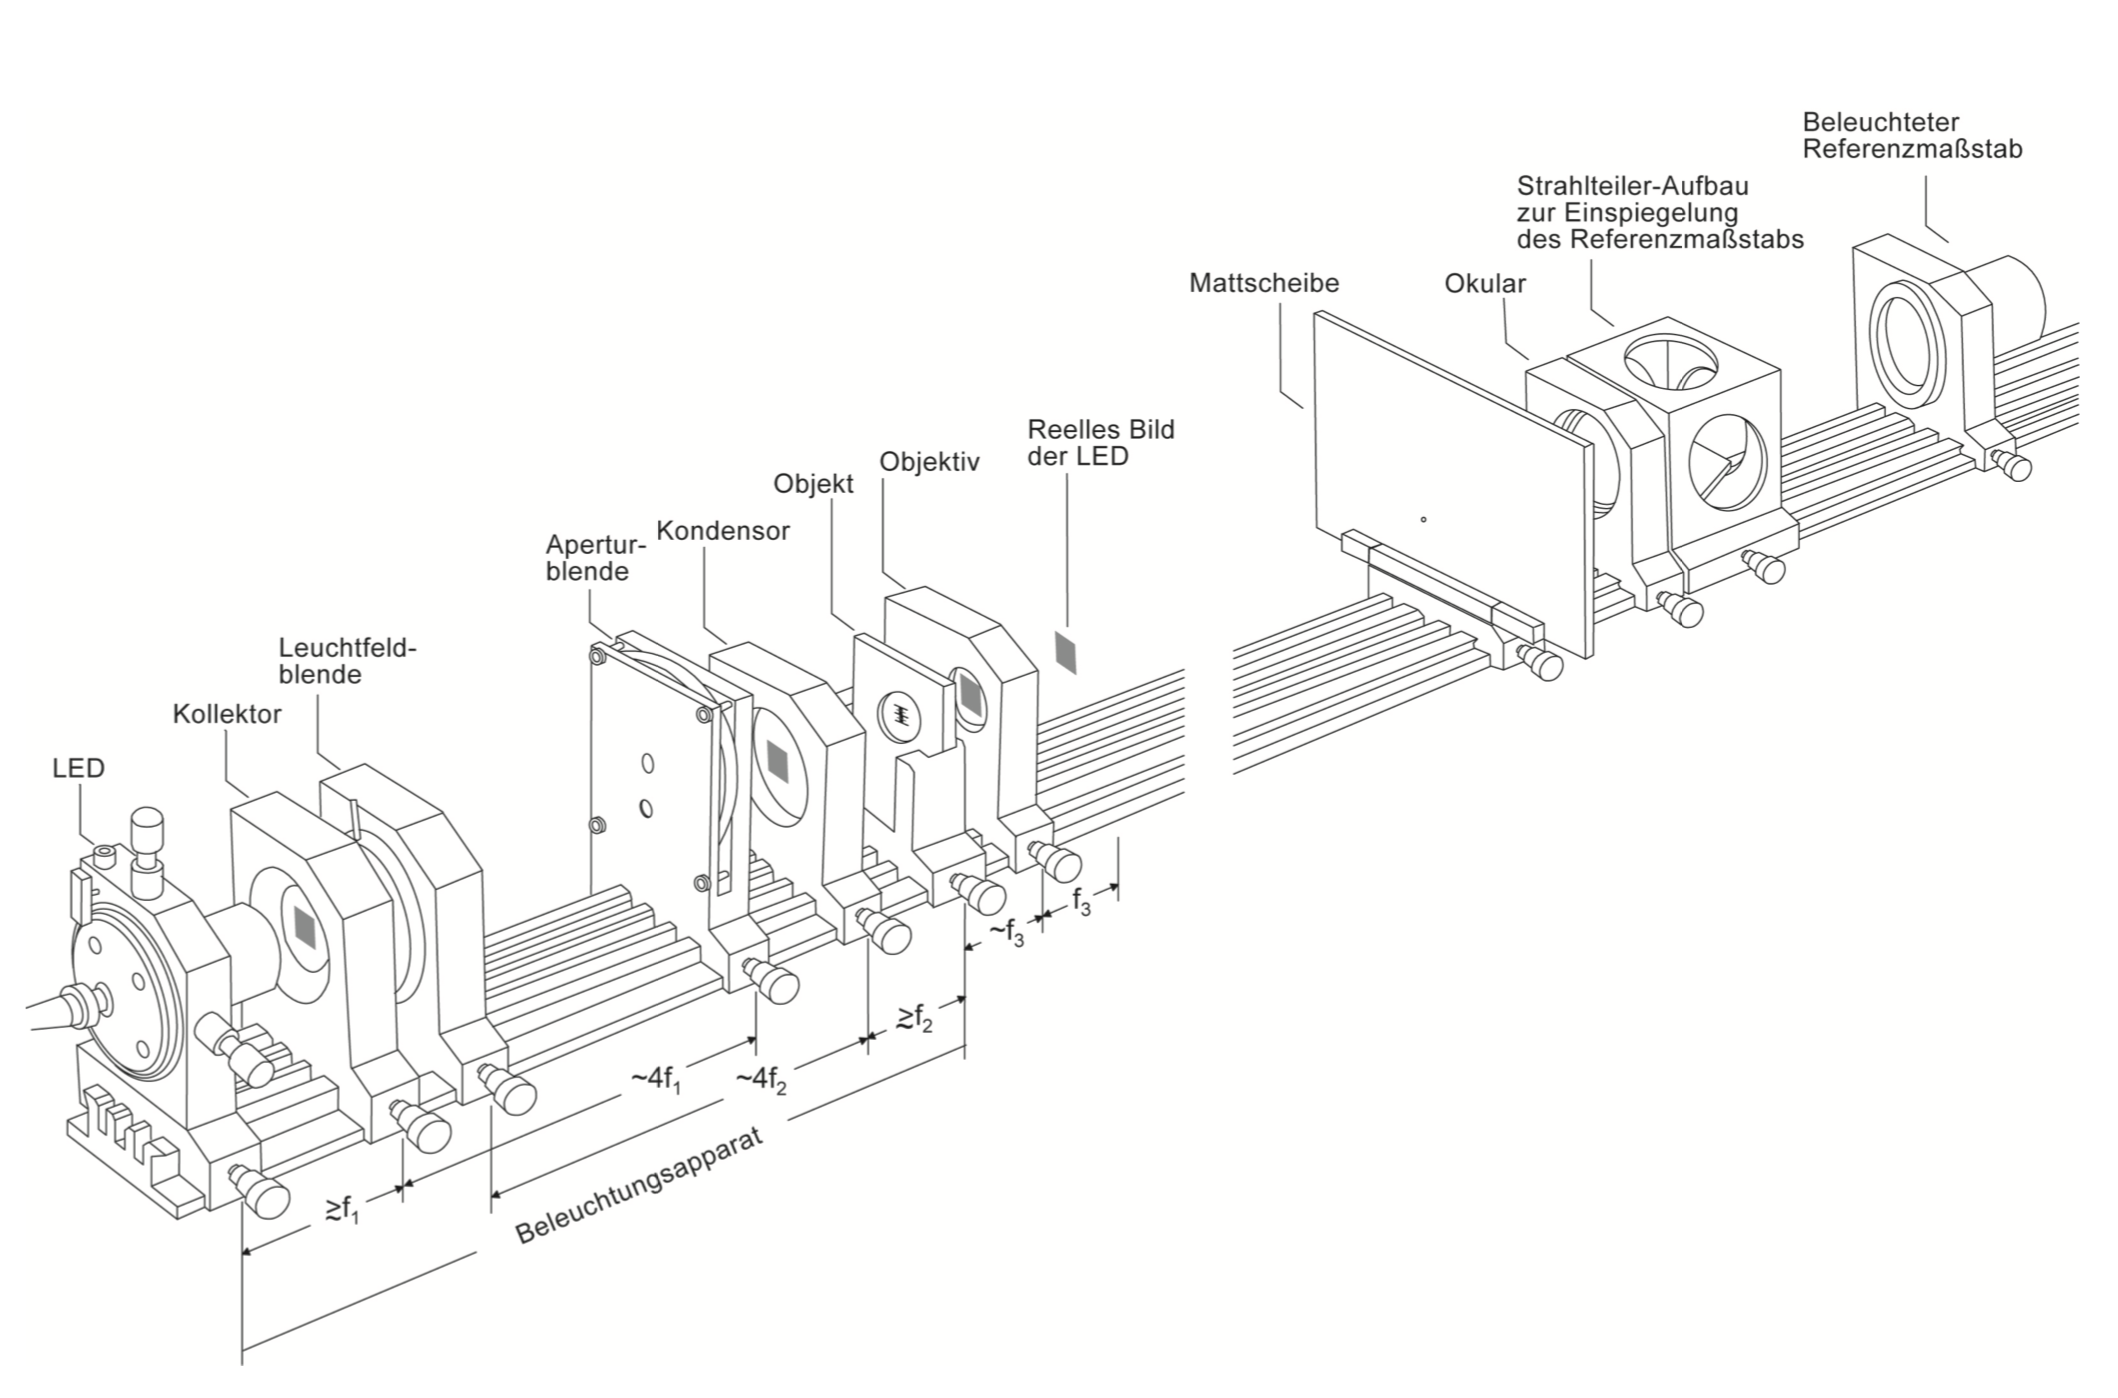
\includegraphics[width=0.8\textwidth]{pork}}
\caption{Versuchsaufbau \cite{Anleitung}}
\label{Pic:X}}
\end{figure}


\section{Durchführung}

\subsection{Aufgabe 1}

Zuerst wurde als Objekt das Dia mit dem Gittermuster vor dem Objektiv gestellt, bei der Position 25.0\,cm. Zunächst wird nach der Lichtquelle eine Kollektorlinse platziert, welches so verschoben wird, dass das Objekt gut ausgeleuchtet wird und keine sphärischen oder chromatischen Abberationen auftreten. Dies war bei der Position 10.9\,cm Als nächstes wird die Aperaturblende eingesetzt, diese verändert die Helligkeit der Beleuchtung am Objekt. Die Aperaturblende muss dafür vor dem Objekt platziert werden and der Position 19.1\,cm. Abschliessend wird die Leuchtfeldblende so nah wie möglich an die Kollektorlinse platziert (Position 12.9\,cm), dies ermöglicht es den ausgeleuchteten Bereich am Objekt zu ändern, ohne die Helligkeit zu beeinflussen. 

\subsection{Aufgabe 2}

In diesem Teil wird die Beleuchtung durch Abstimmung des Beleuchtungsstrahlengangs und des Abbildungsstrahlengangs optimiert. Unsere optischen Komponenten waren schon aus dem ersten Teil gut platziert, sodass nur noch die Kondensorlinse genau eine Brennweite also 4\,cm hinter der Aperaturblende gesetzt werden musste.

\subsection{Aufgabe 3}

Zuerst wird das Objekt ausgetauscht mit der Mikrometerskala bedrucktem Dia. Dann wird mit einem Massband die Bildweite ($b$) und Gegenstandweite ($g$) gemessen. Dann wird die Bildgröße ($B$) und Gegenstandgröße ($G$) mit dem Geodreieck gemessen. 

Zunächst wird der Schirm entfernt und das Okular 5\,cm hinter der Halterung platziert, dann wird der Strahlenteiler direkt neben dem Okular eingesetzt. Mit diesem Aufbau wird zunächst die Vergrösserung des Okular gemessen. Hierfür werden drei Verfahren verglichen. Ein mal durch einsetzen des semi-transparenten Schirms auf dem ein reelles Zwischenbild der Mikrometerskala erscheint. Durch den Strahlenteiler wird dieses Zwischenbild mit der Referenzskala überlagert. Die Vergrößerung wird notiert und der Schirm wird mit der Mattscheibe ersetzt. Die Skala auf der Rückseite des Schirms wird beleuchtet und wieder mit der Referenzskala verglichen. In dem dritten Verfahren wird der Schirm entfernt und das Bild direkt mit der Referenzskala verglichen. 

\subsection{Aufgabe 4}

Um die räumliche Auflösung des Mikroskops zu bestimmen wird zunächst das Abbe-Kriterium verwendet. Hierfür wird ein verstellbarer vertikaler Spalt hinter dem Objektiv gesetzt. Die Mattscheibe wird wieder eingebaut. Dann wird der Spalt so lange verringert bis die Striche and der abgebildeten Skala gerade nicht mehr getrennt wahrgenommen werden können. Um die Spalt breite dann zu bestimmen wird das Objekt entfernt und mit dem Spalt ersetzt. Der Spalt wird dann an dem Schirm abgebildet und kann gemessen werden wobei die im Teil 3 bestimmte Vergrösserung verwendet wird. 

\subsection{Aufgabe 5}

Zuletzt wurde das Objekt wieder eingesetzt und der Spalt entfernt. Dann wurde das Dia mit dem Gitter wieder eingebaut und Abbildungsfehler betrachtet. Hier traten leichte sphärische und chromatische Abberationen auf. Dann wurde die Vergrößerung unseres Aufbaus mit der des kommerziellen Mikroskops verglichen. 

\section{Auswertung}

Um die Vergr"o\ss erung des Mikroskops, die Korrektheit des Aufbaus und die Theorie zu "uberpr"ufen, berechnen wir zuerst den gemessen Abbildungsma\ss stab des Objektivs $\beta$ mittels (\ref{eq:4}). Mit den bestimmten $B=(98\pm0.2)\,$mm und $G=5\,$mm erhalten wir:
\[\beta=19.60\pm0.04\]
F"ur den Fehler k"onnen wir hier einfach
\[
\frac{\Delta\beta}{\beta}=\sqrt{\left(\frac{\Delta B}{B}\right)^2+\left(\frac{\Delta G}{G}\right)^2}
\]
bestimmen.\\
Dann berechnen wir die Vergr"o\ss erung des Mikroskops. Wir rechnen
\[V_\textrm{M}=\frac{B}{G}\frac{d_1}{d_2}\]
mit $d_1$ als die am Referenzma\ss stab gemessene L"ange und $d_2$ die Gr"o\ss e des Bilds. Als Werte haben wir $d_1=(10.00\pm0.03)\,$mm und $d_2=(3.00\pm0.03)\,$mm. Wir erhalten:
\[V_\textrm{M}=(65.3\pm0.7)\]
Zur Fehlerberechnung kann man hier die vereinfachte Form der gau\ss schen Fehlerfortpflanzung verwenden:
\[
\frac{\Delta V}{V}=\sqrt{\left(\frac{\Delta d_1}{d_1}\right)^2+\left(\frac{\Delta d_2}{d_2}\right)^2}
\]
Um dann zum Vergleich den theoretischen Wert zu finden, rechnen wir laut (\ref{eq:5}) einfach
\[V_\mathrm{M}=\frac{b}{g}\frac{s_0}{f_2}\]
Unsere Messwerte lauten
\begin{itemize}
\item $b=(826\pm1)\,$mm
\item $g=(42.036\pm0.004\,$mm
\end{itemize}
mit $s_0=250\,$mm und $f_2=80\,$mm. Zur Berechnung von $g$ rechnen wir
\[
g=\left(\frac{1}{f_1}-\frac{1}{s_{\mathrm{Ok}}-f_4-s_{\mathrm{Obj}}}\right)^{-1}.
\]
Dies folgt aus
\[\frac{1}{f}=\frac{1}{g}+\frac{1}{b},\]
also
\[g=\left(\frac{1}{f}-\frac{1}{b}\right)^{-1}.\]
Partielle Ableitungen lauten dann:
\[
\frac{\partial g}{\partial f}=\frac{b^2}{(b-f)^2}
\]
\[
\frac{\partial g}{\partial b}=-\frac{b^2}{(b-f)^2}
\]
\[
\Delta g=\sqrt{\left(\frac{\partial g}{\partial b}\Delta b\right)^2+\left(\frac{\partial g}{\partial f}\Delta f\right)^2}
\]
Wir erhalten also
\[V_\mathrm{M}=61.4\pm0.1\]


Zudem wollen wir noch mittels des zuvor erw"ahnten Abbe-Kriteriums den kleinsten noch aufl"osbaren Abstand $\delta$ bestimmen und mi dem Strichabstand auf dem Objektmikrometer vergleichen.

Bestimmt haben wir $\beta=20.38\pm0.03$ und $B=(9.8\pm0.2)\,$mm. F"ur den Fehler finden wir dann mit
\[\Delta s=s\sqrt{\left(\frac{\Delta B}{B}\right)^2+\left(\frac{\Delta\beta}{\beta}\right)^2}\]
unseren Fehler auf $s$. Den Wert von $s$ selbst berechnen wir mit
\[s=\frac{B}{\beta}\]
und erhalten
\[s=(0.471\pm0.001)\,\mathrm{mm}.\]
Dazu wollen wir noch unser $\alpha$ berechnen. Wir nutzen eine geometrische Absch"atzung und rechnen
\[\alpha\approx\arctan\left(\frac{s}{f}\right)\approx\frac{s}{f}\]
Wir erhalten $\alpha=(0.01178\pm0.00003)$\,rad. Fehler wird hier analog zu vorherigen mit gau\ss scher Fehlerforpflanzung berechnet.

Wir rechnen jetzt mit (\ref{eq:8}), $n=1$ und $\lambda=540\,$nm $\delta$ aus, wieder mit Fehlerfortpflanzung f"ur die Fehlerberechnung. Unser Ergebnis lautet dann:
\[\delta\approx(2.796\pm0.007)\times10^{-5}\,\mathrm{m}\]

\section{Diskussion}

Um unsere Messwerte auf Vertr"aglichkeit zu "uberpr"ufen, nutzen wir die bekannte $t$-Funktion
\begin{equation}
t=\frac{\vert x_n-y_n\vert}{\sqrt{x_s^2+y_s^2}}\label{eq:6}
\end{equation}
Wir erhalten f"ur unsere oben bestimmten Werte $t=5.58$. Dies ist au\ss erhalb des erw"unschten Bereichs von $t<2$, was Unvertr"aglichkeit impliziert.

Erstaunlich ist dieses Resultat jedoch nicht. Es ist durchaus m"oglich, dass aufgrund von mangelnder Erfahrung die Gr"o\ss en schlecht abgelesen wurden. Eventuell sollten also Fehler gr"o\ss er abgesch"atzt werden.

Systematische Fehler sind hier erstmal, dass nicht klar ist, ob unsere $f$-Werte korrekt sind, da diese vorgegeben wurden. Au\ss erdem ist es durchaus m"oglich, dass die Angaben auf dem Referenzma\ss stab und dem Objekt nicht richtig sind. 

Zur Verbesserung k"onnte man hier in den Halterungen Schlitze einbauen, durch welche man die genaue Position der einzelnen Ger"ate identifizieren k"onnte. Auch w"urde helfen, wenn die Halterung f"ur die Objekte d"unner w"are, sodass die Objekte nicht nach links und rechts rutschen k"onnten, da dies auch die Sch"arfe beeinflusst.

Um noch unseren Wert f"ur die Aufl"osungsbegrenzung zu "uberpr"ufen vergleichen wir diesen mittels (\ref{eq:6}) mit dem Strichabstand $x=5\times10^{-5}\,$m und erhalten $t=315$. Dies impliziert starke Unvertr"aglichkeit. Es ist also wahrscheinlich, dass hier gr"o\ss ere Fehler stattfanden. Wie zuvor ist es aber am wahrscheinlichsten, dass schlecht bzw. falsch abgelesen wurde.

\vfill

%\section{Anhang: Tabellen und Diagramme}
%
%\begin{table}[h]
%\centering
%\caption{XXXX} \vspace{11pt}
%$\begin{array}{l}
%\textrm{Unsicherheiten:}\\
%\textrm{XXXX: } \pm XX \textrm{XX}\\
%\end{array}$
%\begin{tabular}{ccc}
%\toprule
%\textrm{XXXX}/\textrm{XX} & \textrm{XXXX}/\textrm{XX} & \textrm{XXXX}/\textrm{XX} \\
%\midrule 
%2 & 0.26 & 0.23\\
%\hline
%4 & 0.33 & 0.25\\
%\hline 
%5 & & 0.3\\
%\hline 
%6 & 1.25 & 0.83\\
%\hline 
%8 & 3.9 & 0.83\\ 
%\hline
%9 & 4.75 & 4.6\\ 
%\hline
%10 & 4.7 &\\ 
%\bottomrule
%\end{tabular}
%\phantom{$\begin{array}{l}
%\textrm{Unsicherheiten:}\\
%\textrm{XXXX: } \pm XX \textrm{XX}\\
%\end{array}$}
%\label{Tab:X}
%\end{table}

%\begin{figure}[p]
%\centering
%\fbox{\includegraphics[width=0.8\textwidth]{NAME}}
%\renewcommand\thefigure{BX}
%\caption[XXXX]{XXXX}
%\label{Abb:X}
%\end{figure}

\begin{thebibliography}{9}
%\bibitem{Uncertainties}''Correlations between variables are automatically handled, which sets this module apart from many existing error propagation codes.'' - https://pythonhosted.org/uncertainties/
\bibitem{Anleitung} Physikalisches Institut der Albert-Ludwigs-Universität Freiburg (Hrsg.) (08/2018): Versuchsanleitungen zum Physiklabor für Anfänger*innen, Teil 1, Ferienpraktikum im Sommersemester 2018.
\end{thebibliography}

\end{document}
